\section{Constraining the tensor power spectrum}
The first analysis we conducted aims to show how data from a future PIXIE-like experiment can improve current constraints on the tensor-to-scalar ratio $r$. Therefore, to begin we reproduced the constraints set by BICEP/\emph{Keck} 2018 on the tensor-to-scalar ratio for nearly scale invariant power spectra ($n_t=0$) 
\begin{equation*}
r_{0.05}< 0.035\qquad \text{at 95\% CL.}
\end{equation*}
We then used the two-scale parametrization,  at $k_1=0.02$ Mpc$^{-1}$ and $k_2=0.005$ Mpc$^{-1}$, to set the following 95\% CL upper limits with BICEP/\textit{Keck} 2018 likelihood only (red plot in Figure \ref{fig:r_const}):
\begin{equation*}
r_{0.005}<0.060 \,, \qquad r_{0.02}<0.103 \,.
\end{equation*}
The difference with the 95\% CL upper limits obtained in \cite{Paoletti_2022}:
\begin{equation*}
r_{0.005}<0.030 \,, \qquad r_{0.02}<0.098 \,.
\end{equation*}
has to be ascribed to the use of Planck data in \cite{Paoletti_2022}.
%\begin{figure}[h!]
%        \centering
%        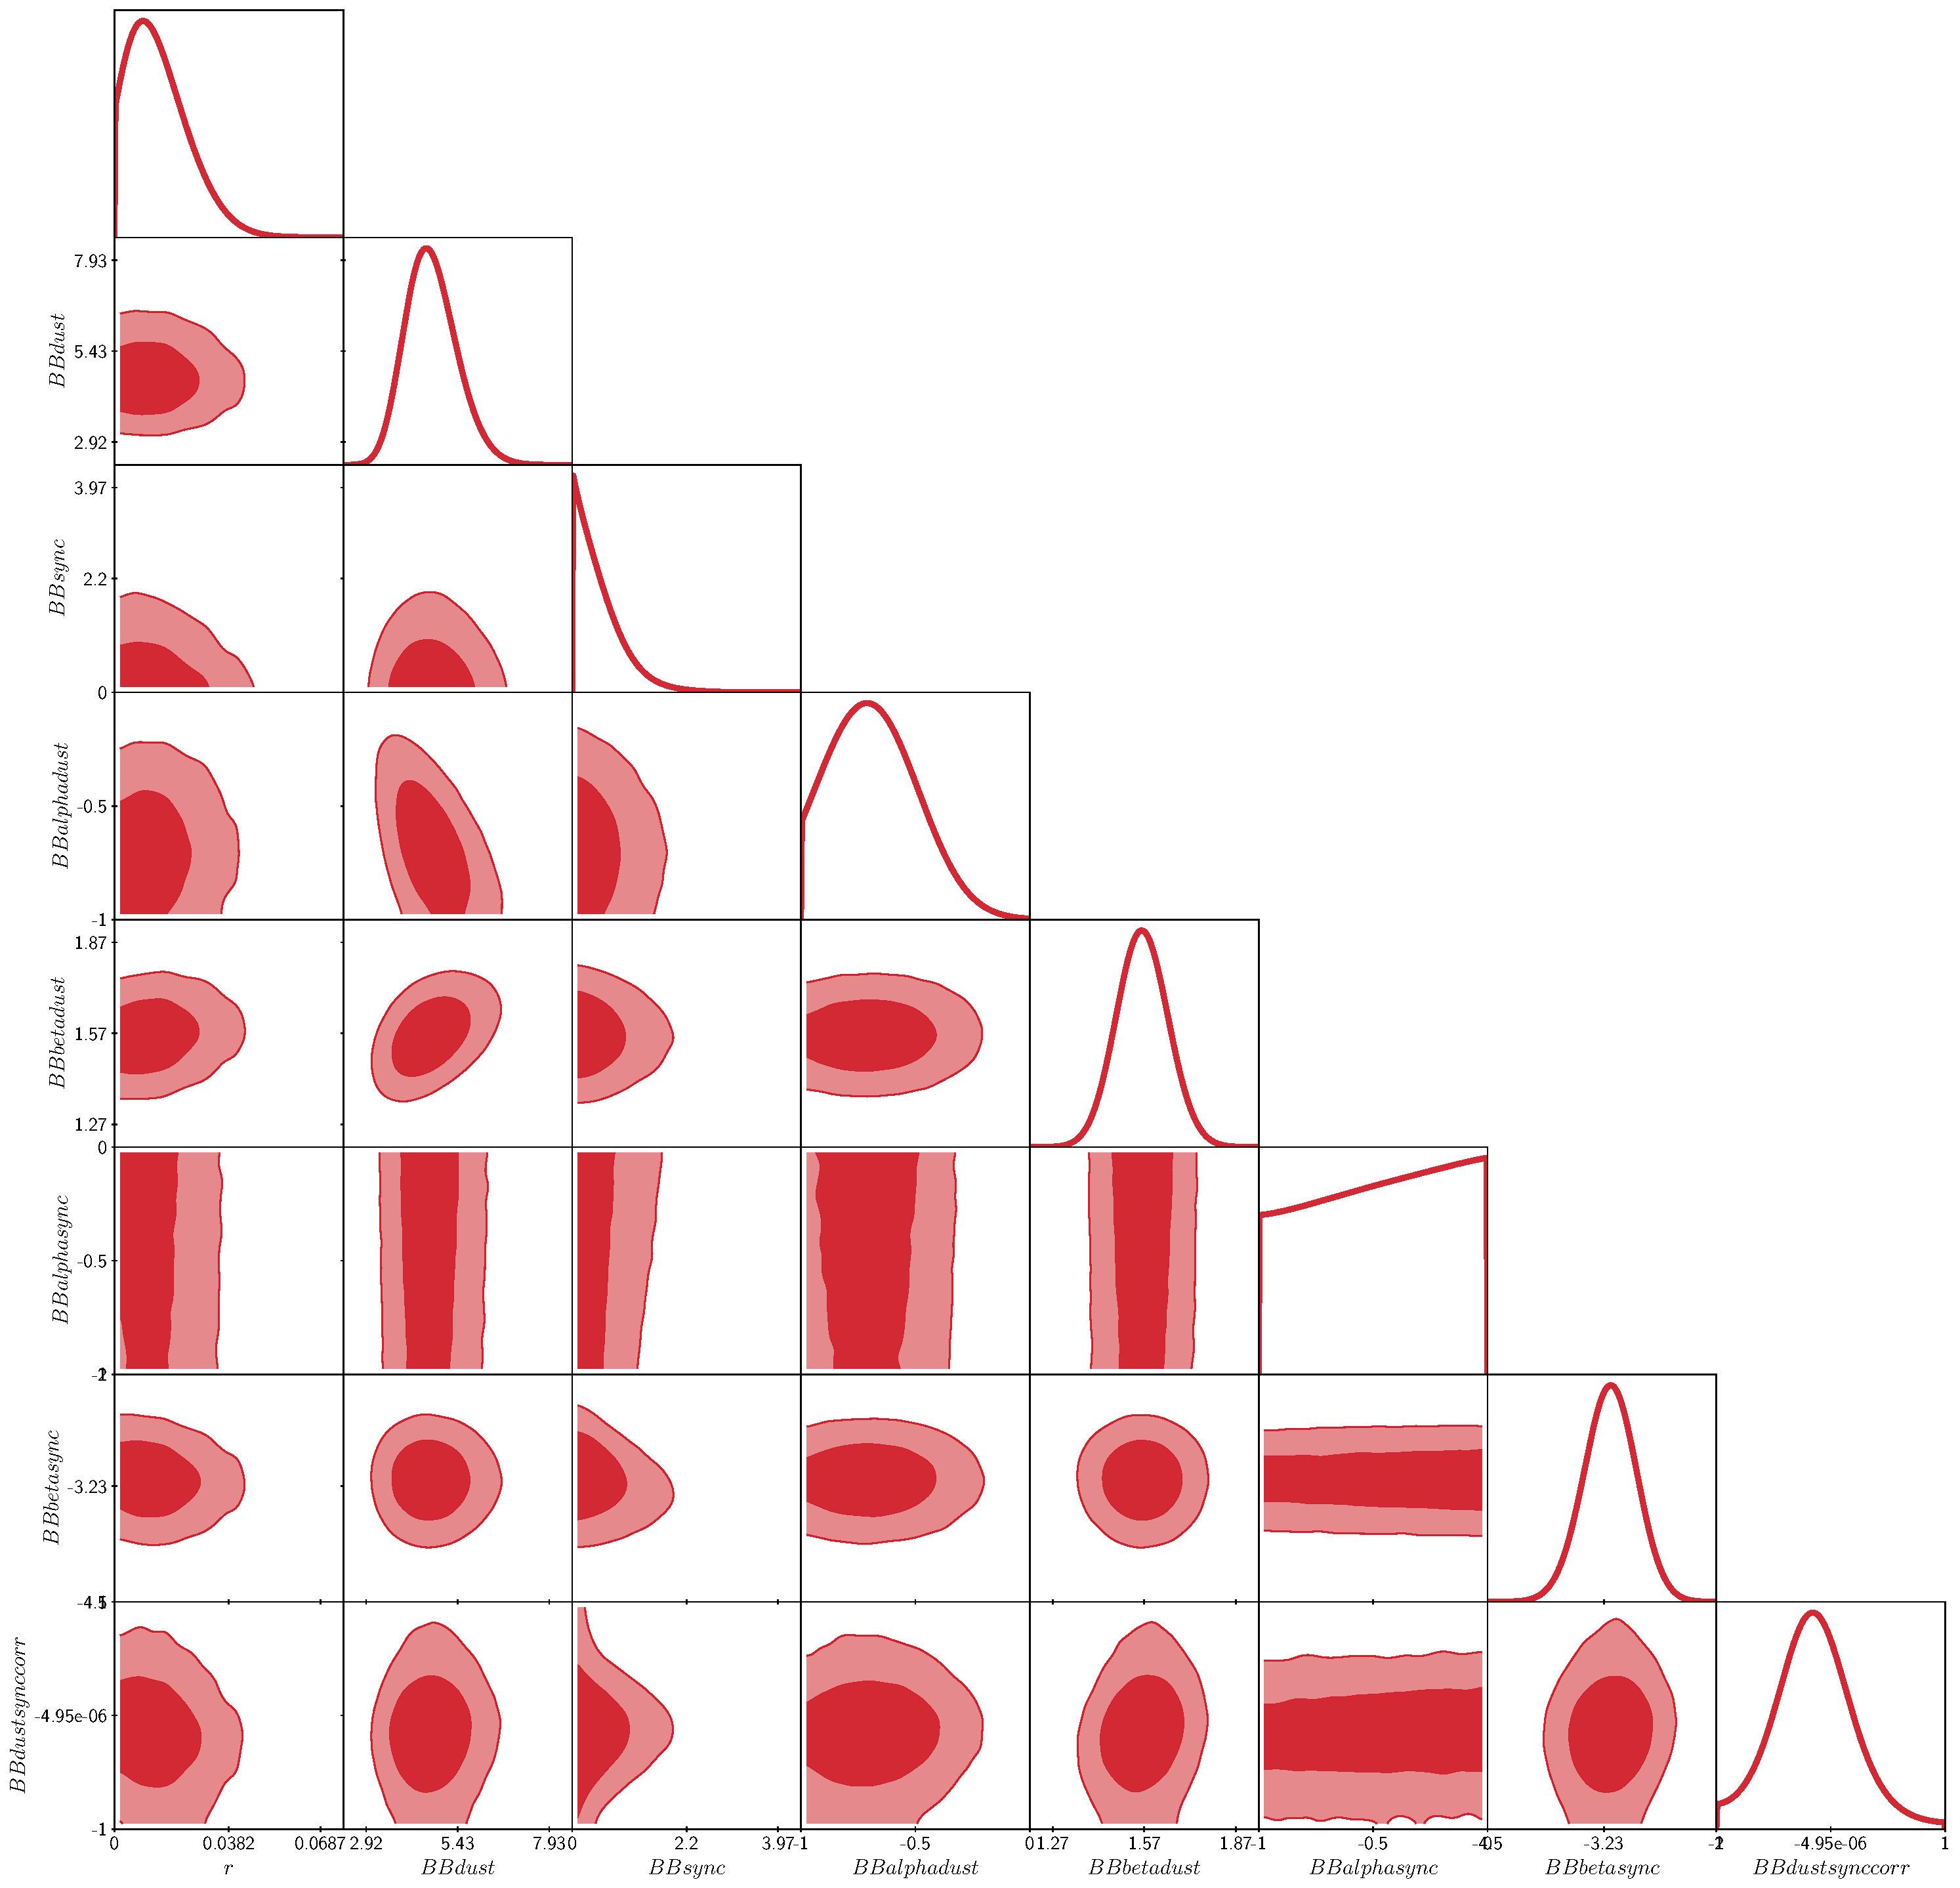
\includegraphics[width=.75\textwidth]{Constraints/BK18_triangle.pdf}
%        \caption{Posterior distributions of the tensor-to-scalar ratio $r$ at the pivot scale $k_\star=0.05$ Mpc$^{-1}$and of the nuisance parameters of BICEP/\emph{Keck} 2018.}
%        \label{fig:r18_const}        
%    \end{figure}

We then moved to the preparation of the PIXIE-like setup: we produced a fiducial set of data using $\Lambda$CDM parameters of \cite{planck2018results} with $r=0$, which corresponds to a non-detection of spectral distortions. We then run three MCMC simulations fixing all the $\Lambda$CDM parameters and varying the two tensor-to-scalar ratios on a flat prior between $[0,1]$. In this analysis we combined the BICEP/\emph{Keck}18 likelihoods with our PXIE-like simulation and we allowed for different PIXIE foreground nuisance parameters to vary, to study how constraints change assuming a perfect knowledge of the foreground. In particular, we first allowed for all the foreground parameters to vary (blue plot in Figure \ref{fig:r_const}), then we fixed them all except for the y amplitude from reionization (green plot in Figure \ref{fig:r_const}) and lastly we fixed all of them (orange plot in Figure \ref{fig:r_const}). 

\begin{figure}[t]
        \centering
        \begin{subfigure}[b]{.49\textwidth}
            \centering
            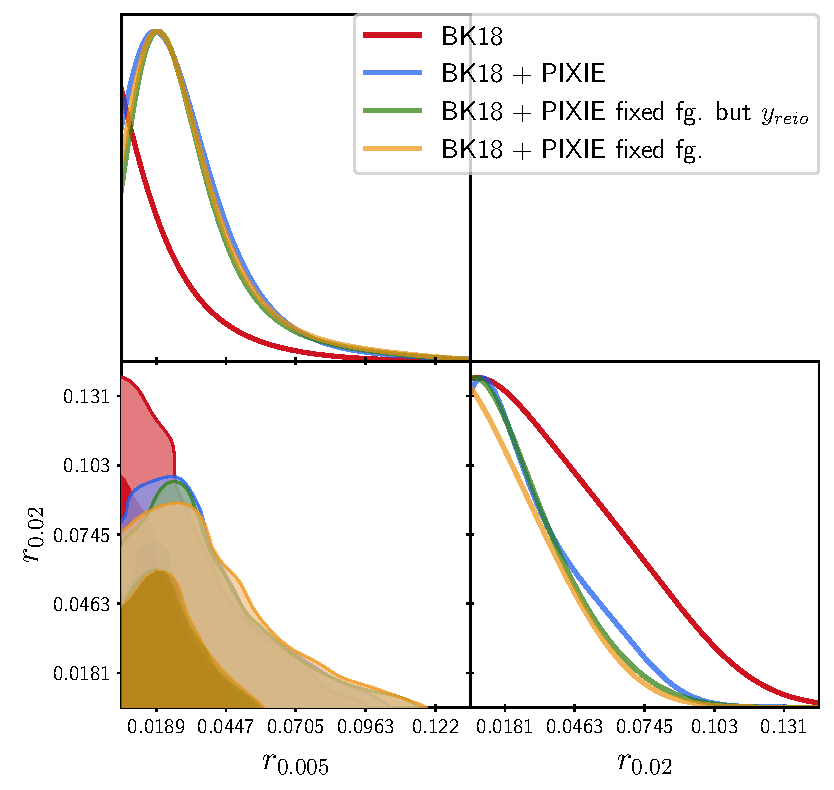
\includegraphics[width=1\textwidth]{Constraints/BKPIXIE.pdf}
            \caption{Posterior of $r_{0.02}$ and $r_{0.005}$.}
            \label{fig:r_const} 
        \end{subfigure}
        \begin{subfigure}[b]{.49\textwidth}
            \centering
            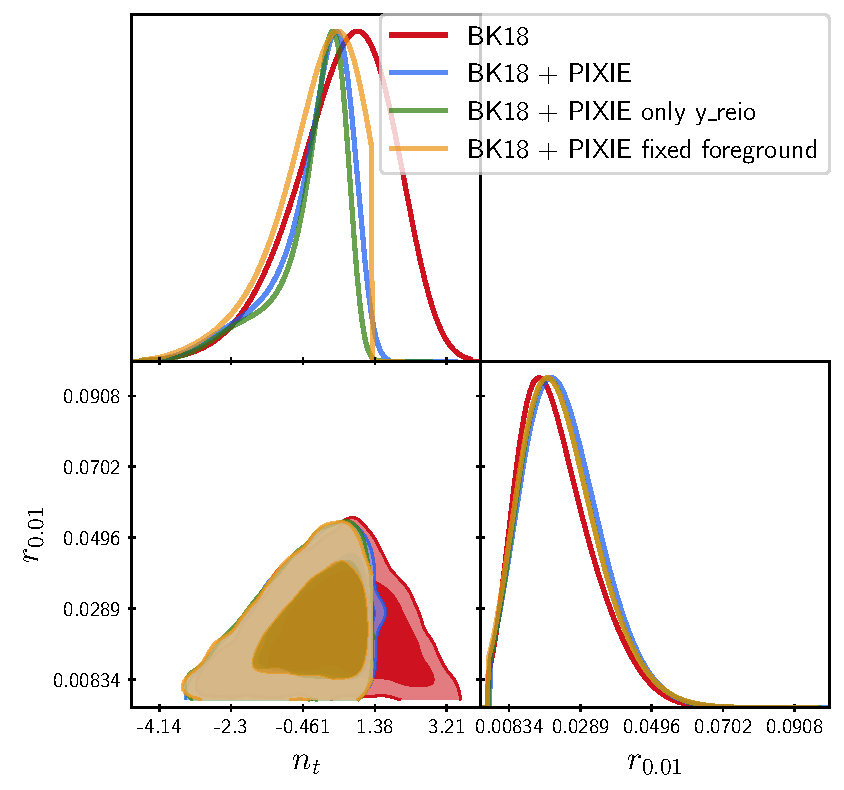
\includegraphics[width=1\textwidth]{Constraints/nt.pdf}
            \caption{Posterior of $n_t$ and $r_{0.01}$.}
            \label{fig:nt_const} 
        \end{subfigure}
        \caption{Posterior distributions of the tensor-to-scalar ratio $r$ at two different scales $k_1=0.02$ Mpc$^{-1}$ and $k_2=0.005$ Mpc$^{-1}$ (a) and of the spectral index $n_t$ and $r$ at $k=0.01$ Mpc$^{-1}$ (b). The red contours are obtained using only data from BICEP/\textit{Keck} 2018 \cite{Ade_2021} while the other contours are obtained combining BICEP/\textit{Keck} 2018 with simulated data from a PIXIE-like experiment. The blue contours are obtained by marginalizing over all the foreground/nuisance parameters, the green one by assuming a perfect knowledge of all of these parameters except $y_\text{reio}$ and the orange one including this last one.}       
    \end{figure}
Figure \ref{fig:r_const} shows how combining spectral distortions with CMB polarization anisotropies improves the constraints on $r$ at the larger scale. 
%Indeed, the 95\% CL upper limits we obtained only from BICEP/\textit{Keck} 2018 data
%$$r_{0.005}<0.060,\qquad r_{0.02}<0.103,$$
once PIXIE-like data is included, become 
\begin{align*}
    &r_{0.005}<0.072,\quad &r_{0.02}<0.072\qquad&\text{95\%CL with foreground,}\\
    &r_{0.005}<0.075,\quad &r_{0.02}<0.067\qquad&\text{95\%CL with only $y_{\text{reio}}$,}\\
    &r_{0.005}<0.076,\quad &r_{0.02}<0.065\qquad&\text{95\%CL with fixed foreground}.
\end{align*}
We should also note that fixing the PIXIE nuisance parameters makes the constraint tighter on $r_{0.02}$.\\ 
Moreover, we also translated these results into constraints on the spectral index and on the tensor-to-scalar ratio at a single scale $k=0.01$ Mpc$^{-1}$. 
%\begin{figure}[t]
 %       \centering
 %       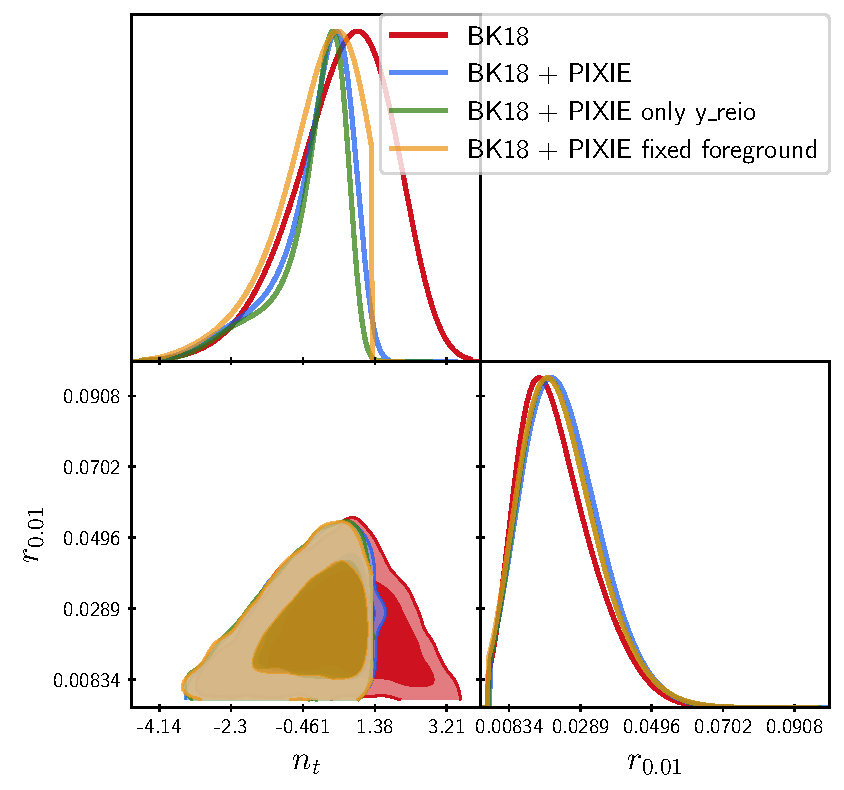
\includegraphics[width=.5\textwidth]{Constraints/nt.pdf}
 %       \caption{Posterior distribution of the tensor-to-scalar ratio $r$ at the scale $k=0.01$ and of the spectral index $n_t$. The red contour is obtained using only data from BICEP/\textit{Keck} 2018 \cite{Ade_2021} while the other contours are obtained combining BICEP/\textit{Keck} 2018 with simulated data from a PIXIE-like experiment. The blue contour is obtained by marginalizing over all the foreground/nuisance parameters, the green one by assuming a perfect knowledge of all of these parameters except $y_\text{reio}$ and the orange one including this last one.}
        %\label{fig:nt_const}        
%\end{figure}
 As we can note from the plot \ref{fig:nt_const}, the contours obtained by our combined analysis are sharply bounded for blue spectral indexes corresponding to detectable $\mu$-distortions (see discussion of Section \ref{sec:num_results}). This behavior is accentuated the most in the orange contour, for which the foreground cannot accommodate bluer tilts.   In this second case, we found that the constraint from with BICEP/\emph{Keck} 2018 alone,
%$$r_{0.01}=0.022^{+0.008}_{-0.013} ,\qquad n_t=0.57^{+1.59}_{-0.96},\qquad \text{68\%CL}$$
$$r_{0.01}=0.022^{+0.021}_{-0.019} ,\qquad n_t=0.57^{+2.39}_{-2.66},\qquad \text{95\%CL}$$
becomes, once we introduce the PIXIE-like data,
%\begin{align*}
%    &r_{0.01}=0.024^{+0.009}_{-0.014} ,\qquad n_t=-0.13^{+1.32}_{-0.45},\quad &\text{68\%CL with foreground }\\
%    &r_{0.01}=0.024^{+0.009}_{-0.014} ,\qquad n_t=-0.22^{+1.30}_{-0.41},\quad &\text{68\%CL with only }y_\text{reio},\\
%    &r_{0.01}=0.023^{+0.009}_{-0.014} ,\qquad n_t=-0.27^{+1.34}_{-0.43},\quad &\text{68\%CL with fixed foreground. }
%\end{align*}
\begin{align*}
    &r_{0.01}=0.024^{+0.022}_{-0.021} ,\qquad &n_t=-0.13^{+1.48}_{-2.31},\quad &\text{95\%CL with foreground }\\
    &r_{0.01}=0.024^{+0.023}_{-0.021} ,\qquad &n_t=-0.22^{+1.44}_{-2.16},\quad &\text{95\%CL with only }y_\text{reio},\\
    &r_{0.01}=0.023^{+0.024}_{-0.021} ,\qquad &n_t=-0.27^{+1.52}_{-2.17},\quad &\text{95\%CL with fixed foreground. }
\end{align*}
 Overall, as we already noted blue spectral indexes ($n_t\sim1$), which are compatible with detectable tensor-induced spectral distortions, sit perfectly on the upper bound set by our analysis. On the other hand, the most red spectral indexes allowed by BICEP/\emph{Keck} alone ($n_t\sim-3$) are ruled-out by our PIXIE-like experiment.
\begin{figure}[t]
    \centering
\begin{tikzpicture}
  \begin{axis}[
      grid=major,
      xlabel={$k$ [1/Mpc]},
      ylabel={$\mathcal{P}_T$},
      width=12cm, height=7cm,
      xmode = log, ymode = log,
      xmin = 1e-5, xmax = 1e8,
      ymin = 1e-20,
      legend pos = south east,
      legend style={font=\scriptsize},
      error bars/.cd,
  ]
    % Load and plot from the external file
    \addplot [thick, smooth, dashed] table {Constraints/constr_PIXIE_mu.dat};
    \addlegendentry{PIXIE semi-analytical constraint}
    \addplot [thick, smooth, gray] table {Constraints/Pk_blue.dat};
    \addlegendentry{BK18 + PIXIE blue $n_t$ upper limit}
    \addplot [thick, smooth, black] table {Constraints/Pk_red.dat};
    \addlegendentry{BK18 + PIXIE red $n_t$ upper limit};
    \draw[thick, |-|, black] (axis cs: 0.02,1e-30) -- (axis cs: 0.02, 7.842648e-02*2.1684389273e-9);
    \draw[thick, |-|, black] (axis cs: 0.005,1e-30) -- (axis cs: 0.005, 6.733576e-02*2.2762465194e-9);
    \filldraw[gray] (axis cs: 6.5e5,3e-5) circle (1mm)node[black, anchor = south] {\small NANOGrav15};
  \end{axis}
\end{tikzpicture}
\caption{Comparison of the largest and most blue tilted and red tilted (at 68\%CL) power laws allowed  by the constraints set by BICEP/\emph{Keck} 2018 + PIXIE-like analysis (solid lines) and the analytical constraints given by PIXIE (dashed line). In the plot also the constraints on $r_{0.02}$ and $r_{0.005}$ are shown alongside one data point representing the PTAs-probed power spectrum by the NANOGrav collaboration \cite{NANOGrav}. }
\label{fig:analy_const_BK18}
\end{figure}

We also compared the largest and two most blue and red tilted power law power spectra, allowed by the constraints we obtained at 68\% CL. Two errorbars are used to indicate the constraints on $r_{0.005}$ and $r_{0.02}$. As we can see in Figure \ref{fig:analy_const_BK18} the blue tilted power spectrum intercepts the semi-analytical constraint of PIXIE while the red one remains at far lower values. This is consistent with our results: indeed we already noticed that blue power spectra are further constrained by the PIXIE-like data, since for $n_t\sim1$ detectable spectral distortions are produces, while red power spectra are still mainly constrained by CMB polarization.\\ In Figure \ref{fig:analy_const_BK18} we also included data one point that displays the power spectrum associated with the \emph{Pulsar Timing Arrays} (PTAs) signal measured by the NANOGrav15 \cite{NANOGrav} collaboration, in its cosmological interpretation: this simple comparison shows that spectral distortions non-detection would not rule-out this possibility and indeed PTAs could further refine our constraints.

Overall, we showed that spectral distortions induced by primordial gravitational waves can impact the constraint that B-modes of polarization anisotropies put on the primordial tensor power spectrum reducing the allowed parameter space.
This strong synergy between spectral distortions and CMB anisotropies opens for the possibility of further constraining the tensor-to-scalar ratio by adding to our analysis \textit{Planck} data. 
\section{Constraining log-normal bumps}
To conclude we discuss the constraint that can be put on the simple modifications of the power law power spectrum of tensor perturbations. Indeed, it is reasonable to assume that moving towards smaller scales, such as those of spectral distortions, the tensor power spectrum could deviate from the power law we expect at the CMB anisotropies scales. The simplest deviation that we could consider is a log-normal (see Section \ref{sec:primordial_PS}) bump placed in the middle of the $\mu$-distortions window function, e.g. $k_\text{pk}=10$ Mpc$^{-1}$. This kind of bumps can accommodate the constraint on the tensor-to-scalar ratio at CMB anisotropies scales while allowing for a detectable primordial gravitational waves-induced distortion to appear.
In this section we constraint the amplitude of these bumps using simulated data from a PIXIE-like experiment \cite{pixie}.
\begin{figure}[t]
    \centering
\begin{tikzpicture}
  \begin{axis}[
      grid=major,
      xlabel={$k$ [1/Mpc]},
      ylabel={$\mathcal{P}_T$},
      width=12cm, height=8cm,
      xmode = log, ymode = log,
      xmin = 1e-1, xmax = 1e7,
      ymin = 1e-11, ymax = 0,
      legend pos = south east,
      legend style={font=\scriptsize},
  ]
    % Load and plot from the external file
    \addplot [thick, smooth, dashed] table {Constraints/constr_PIXIE_mu.dat};
    \addlegendentry{PIXIE analytical constraint}
    \addplot [thick, smooth, black] table {Constraints/bump.dat};
    \addlegendentry{Power law + bump}
    \addplot [thick, smooth ,gray] table {Constraints/bump_reio.dat};
    \addlegendentry{Power law + bump only $y_{reio}$}
    \addplot [thick, smooth, dotted, gray] table {Constraints/bump_NN.dat};
    \addlegendentry{Power law + bump fixed foreground}
    \filldraw[gray] (axis cs: 6.5e5,3e-5) circle (1mm)node[black, anchor = south] {\small NANOGrav15};
  \end{axis}
\end{tikzpicture}
\caption{Comparison of the largest bumps allowed by our PIXIE-like analysis and the semi-analytical constraints given by PIXIE (dashed line). We also plotted a data point representing the PTAs-probed power spectrum by the NANOGrav collaboration \cite{NANOGrav}. }
\label{fig:analy_const_bump}
\end{figure}

\begin{figure}[ht!]
    \centering
    \begin{subfigure}{0.49\textwidth}
        \centering
        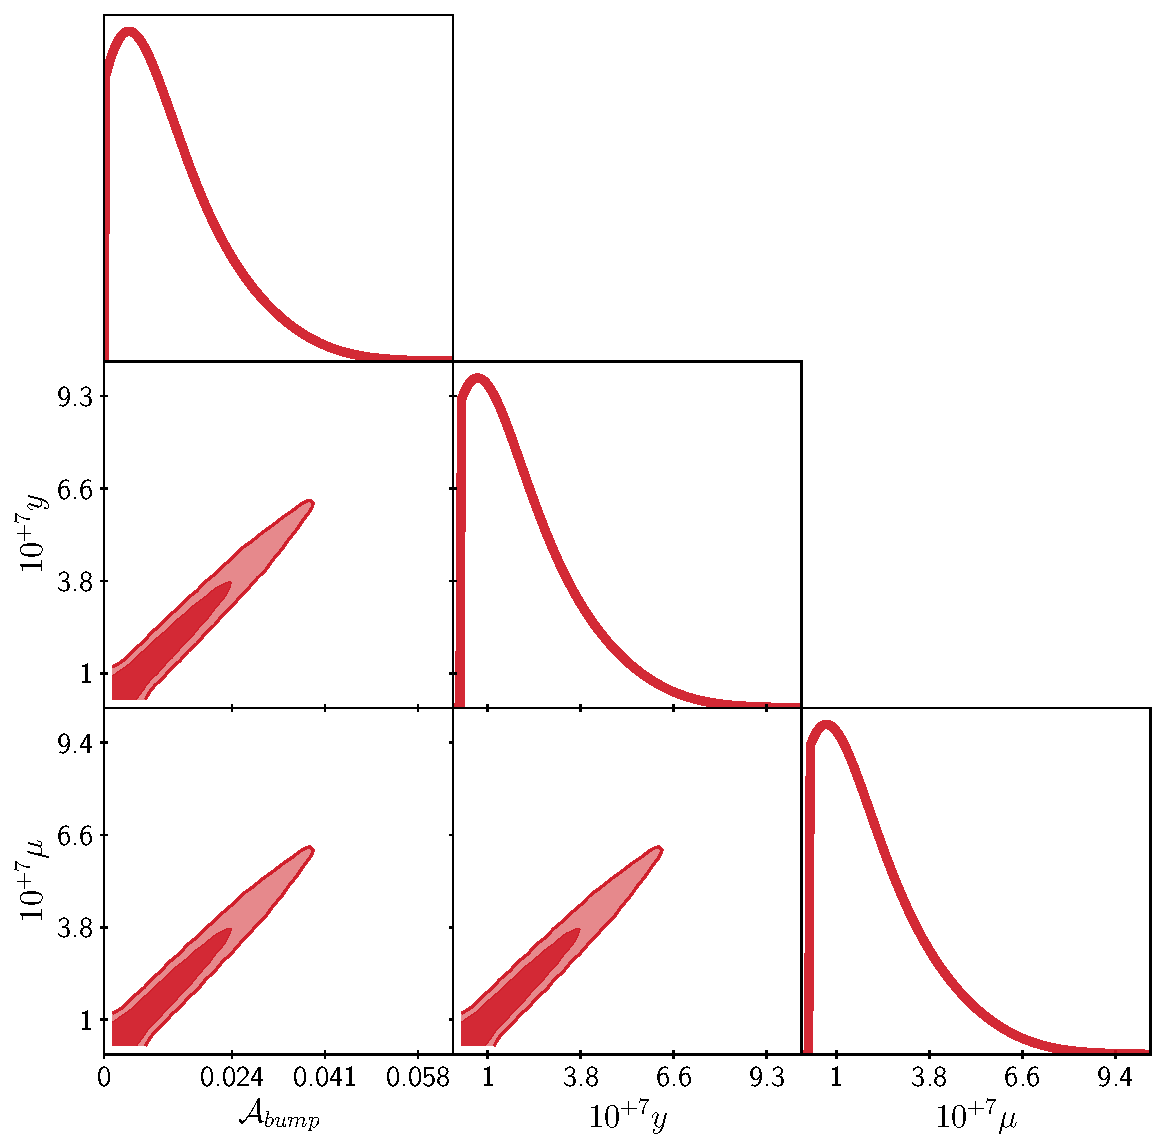
\includegraphics[width=1\textwidth]{Constraints/Lognormal.pdf}
        \caption{Marginalized over the foreground/nuisance}
        \label{fig:LN}        
    \end{subfigure}
    \hfill
    \begin{subfigure}{0.49\textwidth}
        \centering
        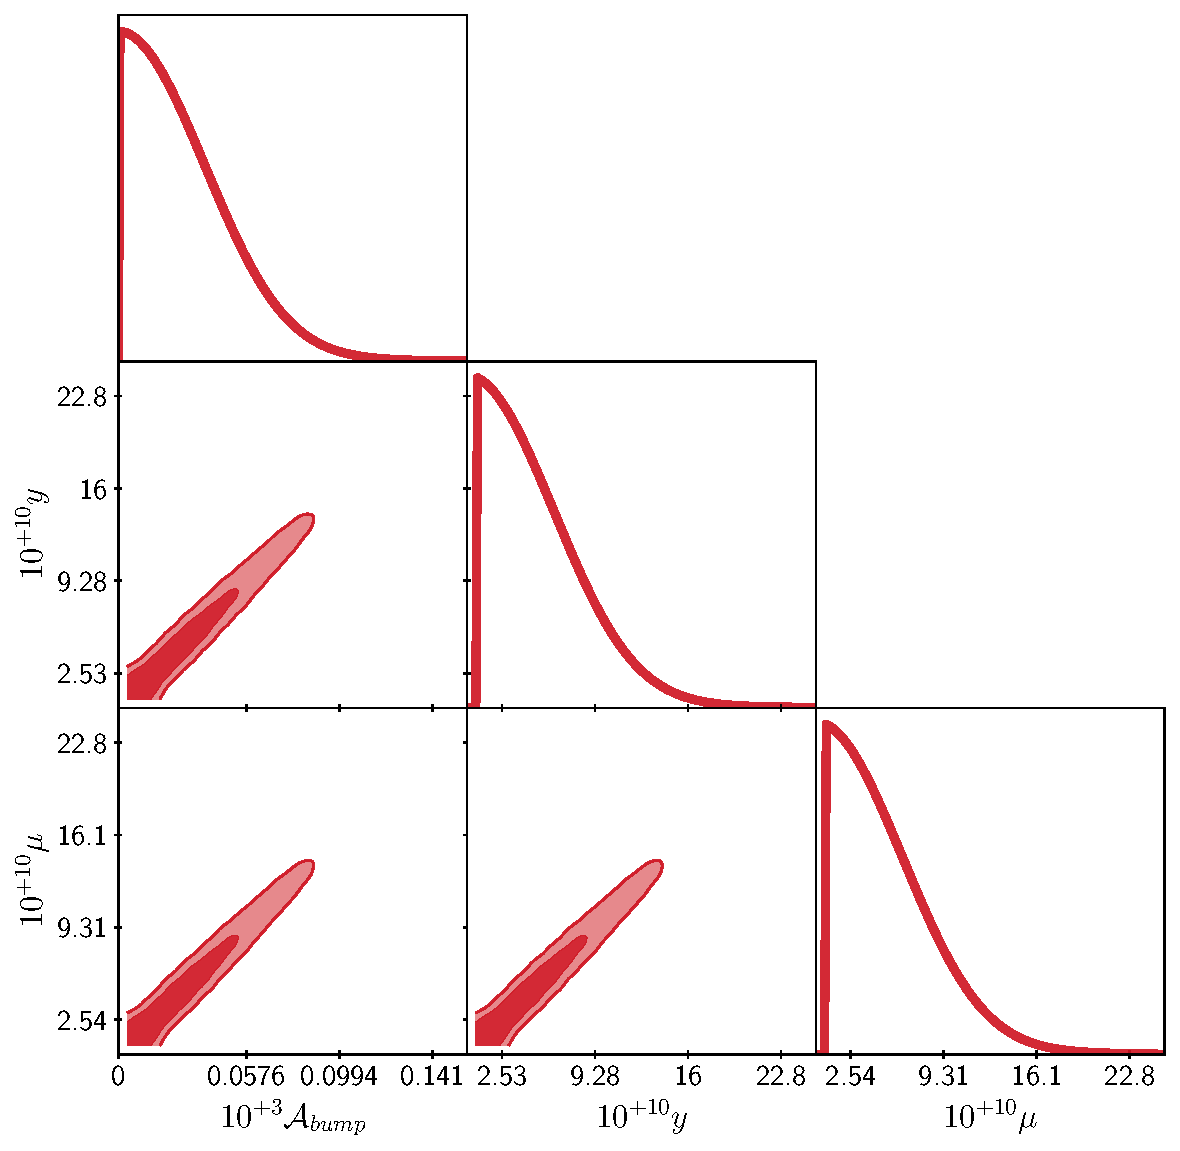
\includegraphics[width=1\textwidth]{Constraints/LN_NN.pdf}
        \caption{Fixed foreground/nuisance}
        \label{fig:LN_NN}        
    \end{subfigure}

    \vspace{1em}

    \begin{subfigure}{0.5\textheight}
        \centering
        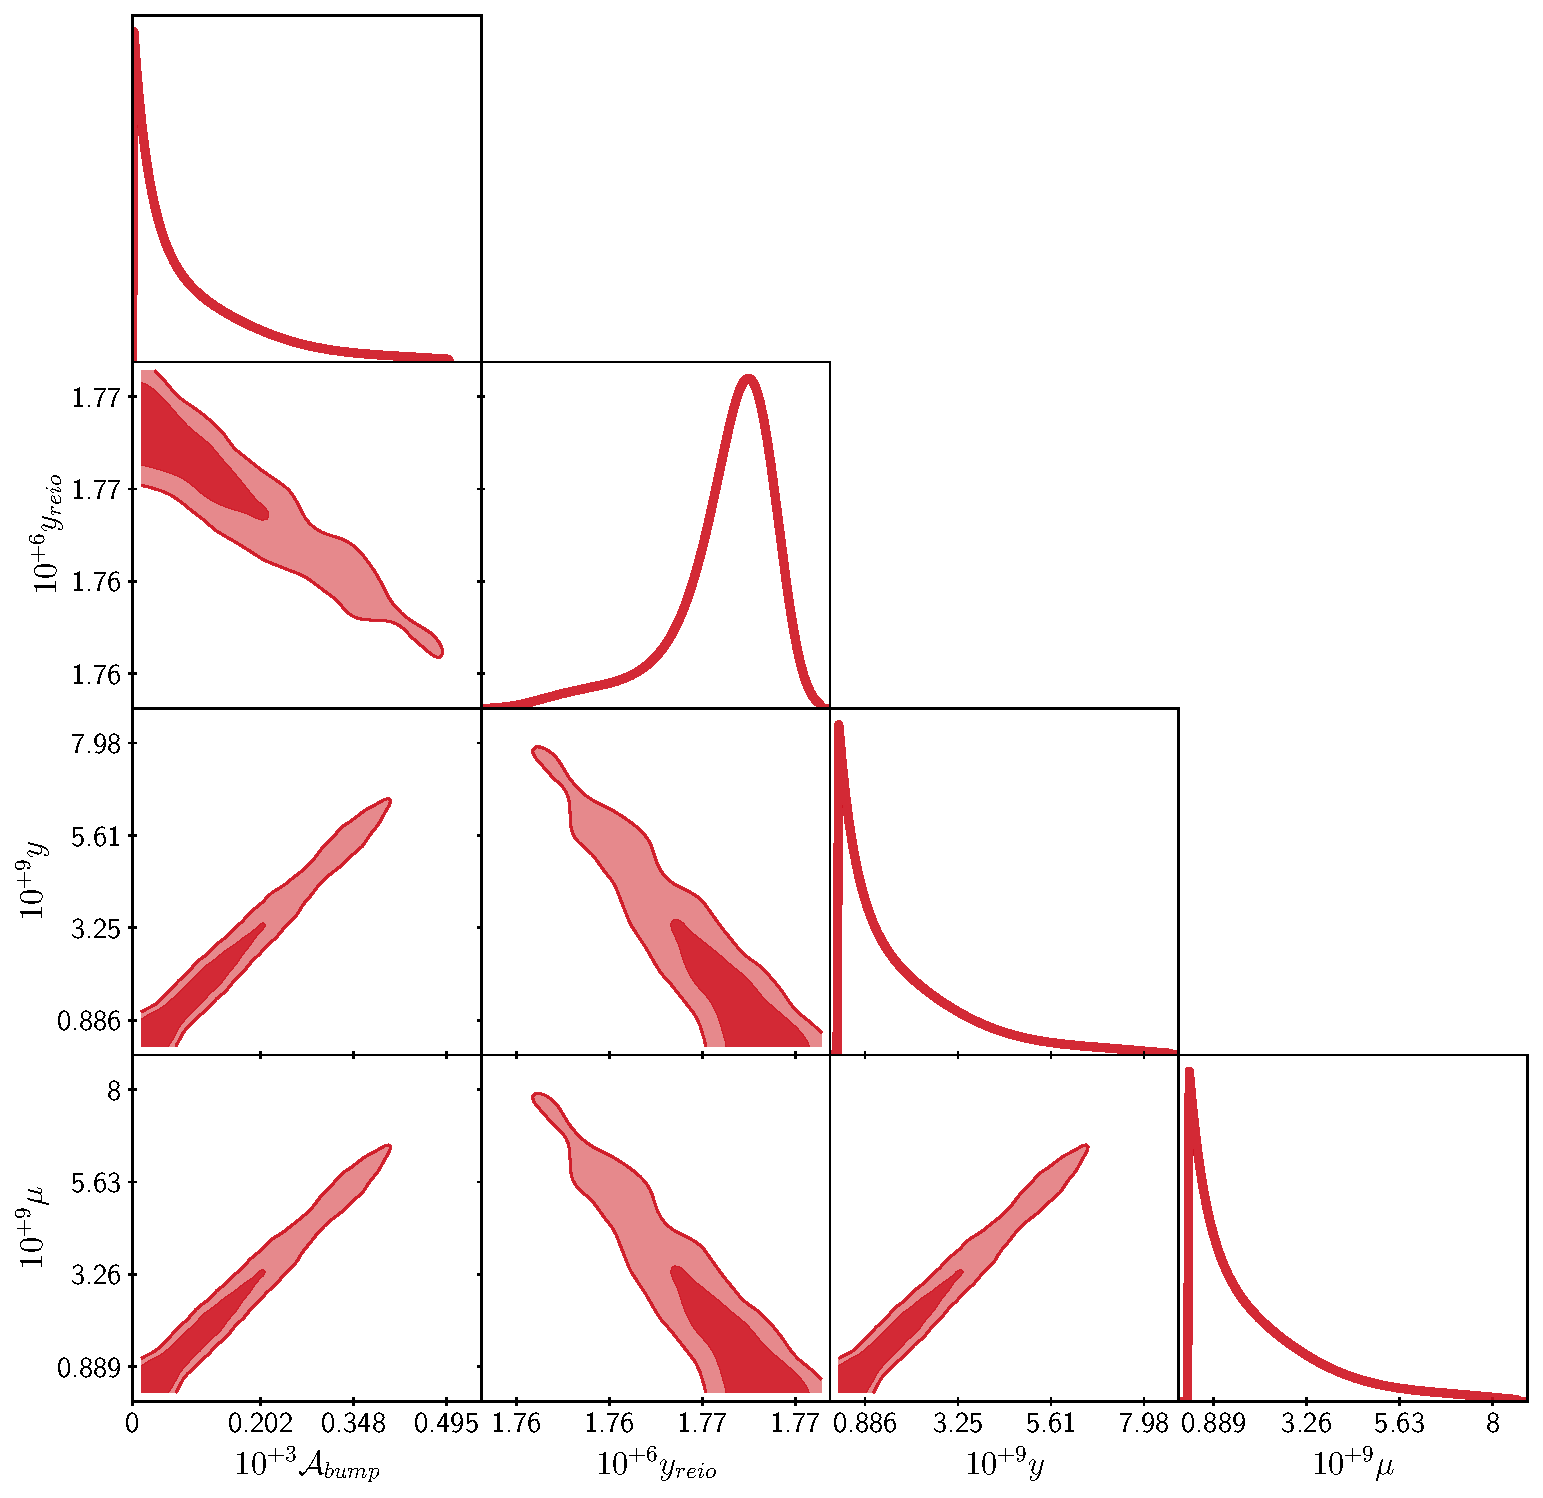
\includegraphics[width=1\textwidth]{Constraints/LN_NN_reio.pdf}
        \caption{Fixed foreground/nuisance except $y_\text{reio}$}
        \label{fig:LN_NN_reio}        
    \end{subfigure}
    \caption{Marginalized posterior distributions for the amplitude of a log-normal bump placed at $k_\text{pk}=10$ Mpc$^{-1}$ with width $\sigma_\text{bump}=0.44$ obtained from a simulated PIXIE-like experiment. The three panels show the results obtained with different assumptions on the nuisance parameters.}
    \label{fig:LN_all}
\end{figure}
We started producing a fiducial set of data from a power spectrum without the bump, with only a power law which satisfies the single field inflation consistency relation $n_t=-r/8$, with $r=0.035$, and the $\Lambda$CDM parameters obtained by the \emph{Planck} collaboration. 
Also for this analysis we conducted three MCMC runs to study how the foreground and the nuisance parameters in Table \ref{tab:nui_pixie} influenced the results. 
The first run (Figure \ref{fig:LN}), in which we marginalized over all the foreground nuisance parameters yielded, for a log-normal template of width $\sigma_\text{bump}=0.44$
an upper value for its amplitude of
$$\mathcal{A}_\text{bump}<3.2\times10^{-2}\qquad\text{at 95\% CL.}$$
In the second run we assumed a perfect knowledge of the nuisance parameters except for the y amplitude generated at reionization (Figure \ref{fig:LN_NN_reio}: in this case tighter constraints were produced 
$$\mathcal{A}_\text{bump}<4.0\times10^{-4}\qquad\text{at 95\% CL.}$$
To conclude, we fixed all the nuisance parameters (Figure \ref{fig:LN_NN}), obtaining
$$\mathcal{A}_\text{bump}<7.7\times10^{-5}\qquad\text{at 95\% CL.}$$

Also for the log-normal template we compared the semi-analytical constraint given by PIXIE with our last three results. In Figure \ref{fig:analy_const_bump}
 we can see that the largest amplitude allowed by the constraint (in figure at 68\% CL) obtained marginalizing over all the nuisance parameters corresponds to a bump that intersects the semi-analytical constraint. Indeed, from Figure \ref{fig:LN} we can see that a distortion $\mu\sim10^{-7}$ is generated, which is in the detectable regime. The other constraints instead correspond to bumps that are a few orders of magnitude lower that the semi-analytical constraint. In this cases the assumption of knowing exactly all or part of the nuisance parameters allows for detections of smaller distortions, which correspond to smaller log-normal amplitudes.\\ We included in this plot, as in Figure \ref{fig:analy_const_BK18},  one data point representing the power spectrum associated to the stochastic background measured by the NANOGrav collaboration from observation of PTAs. We can see that such point could accommodated for similar log-normal templates, placed at a different scale, to the one we studied. This observation opens for the possibility of combining PTAs data with spectral distortions also in this scenario.






